\documentclass[conference]{IEEEtran}
\usepackage{graphicx}
\usepackage{times}
\usepackage{subfigure}
\usepackage{url}

\begin{document}

\title{Six ways to understand monads\\
\small{Experiences from the functional programming course at TU Delft}}

\author{\IEEEauthorblockN{Erik Meijer}
\and
\IEEEauthorblockN{Georgios Gousios}
\IEEEauthorblockA{
Delft University of Technology\\
Delft, The Netherlands\\
Email: {H.J.M.Meijer, G.Gousios, Arie.vanDeursen@tudelft.nl} 
}  
\and
\IEEEauthorblockN{Arie van Deursen}
}
\maketitle

\begin{abstract}

  In the last few years, the popularity of functional programming as a way of
  solving computational problems has increased significantly. While most
  computer science curricula do include a course on functional programming, in
  many cases it is disconnected from practical applications, which is
  precisely where functional programming shines. To fill in this gap, we
  designed a functional programming course that demanded from students to
  learn by experience with real world applications. In this work, we present
  our experiences with conducting this course.

\end{abstract}

\section{Introduction}

Due to a variety of reasons, including the advent of cloud computing, the
rising rate of information production and the necessity to reach the market
fast, currently, large corporations and start-ups alike are investigating
alternative programming and information storage models. As a result, during
the last few years, the practical software engineering field is witnessing a
noticeable shift towards functional programming. Scripting languages, notably
Javascript and Ruby, pioneered the introduction of functional concepts, such as
closures and lambda functions, to mainstream programming. A new wave of
programming languages, developed to overcome the expressiveness and
complexity limitations exhibited in mainstream languages, have promoted
functional constructs, such as type safe pattern matching, higher order
functions and single assignment variables, to first class citizens (Scala).
New, purely functional, languages have emerged to fill in the remaining gaps
(F\#, Clojure), often introducing significant advancements in their field of
specialisation (such as Erlang in distributed fault-tolerant systems).
Finally, large scale information processing systems such as Map-Reduce and
domain specific languages such as LINQ have integrated functional concepts to
ease the expression of computations.

Broadly speaking, functional programming is a style of programming in which the
primary method of computation is the application of functions to arguments.
Among other features, functional languages offer a compact notation for writing
programs, powerful abstraction methods for structuring them, and a simple
mathematical basis that supports reasoning. Many of the advanced techniques in
modern functional languages, such as monads and catamorphisms, are closely based
on principles from category theory such as functors, initial algebras, monads
and Kleisli categories.

While functional programming has been taught for long in computer science
departments~\cite{Joost93}, curricula tend to emphasize functional programming
theory rather than practical applications. Special programming languages are
used to teach functional programming specific concepts, while little connection
is made to how those concepts can be transfered to non-functional languages.
The course at TU Delft attempted to teach functional programming theory in the
classroom and then expect students to apply those concepts in the (non-purely
functional) language of their choice. The course had a very strong teaching by
example focus: students were expected to participate in both in-classroom
exercises, homework assignments and implement a real world system as a final
project.

\section{Challenges}

While planning the course, we dealt with the following challenges related
to the course's organization and content.

\subsection{Heterogeneous background of participants}

The functional programming course is elective at the MSc curriculum. Students
from all departments in the Electrical Engineering, Mathematics and Computer
science faculty are allowed to participate. For practical reasons, the
enrollment to the course was limited to 15 participants. This permitted
us to get to know the students individually and to provide them with
personalized support.

From the students that enrolled, most have received formal introduction to
imperative and object oriented programming in their bachelors curriculum, while
through participation to other courses they had limited exposure to functional
programming (i.e. Map/Reduce~\cite{Dean04} in the web information systems
course). Two of the students were majoring in computer engineering, which meant
that their programming experience was restricted. Several students also had work
experience as programmers as part of their industrial placement or through
participation to start up ventures.

The expected diverse backgrounds of the students guaranteed that no generic
introduction to the topic would be sufficient. For this reason, we decided
to adopt a hands-on-first approach; the students would have to learn by
flexing their programming muscles, instead of being gently introduced to 
the theory through toy examples.

\subsection{Choosing the appropriate topics}

Functional programming is arguably the oldest programming paradigm. In it is
purest form, it is based on a minimalistic theoretical background
($\lambda$-calculus~\cite{Baren84}). Relatively recent
formulations~\cite{Meije91, Wadle93} also introduced concepts from category
theory. While the every day use of functional programming does not necessarily
require the programmer to be aware of the theoretical background, understanding
it usually leads to more elegant algorithmic solutions. Functional
programming teaching is also associated with advanced type systems; the flagship
functional programming languages (Haskell and the {\sc ml} family) both offer
very sophisticated support for types. Consequently, teaching the full spectrum
of functional programming theory and techniques would have been impossible in a
half-semester course; instead we decided to focus on practical aspects of data
processing, transformations and state representation using functional techniques.

\subsection{Choosing the appropriate programming language}

Programming languages, in addition to enabling the programmer to express a
series of instructions to be executed by a computer, affect the programmer's
tough process and consequently her approach towards problem
solving~\cite{Ivers80}.  When teaching a programming course, it is important to
be able to demonstrate concepts without interference by the chosen language's
syntax. However, a non-practical language might have the opposite effect; our
experience has shown that the further a demonstration language is from practical
application, the less important student feel the taught concepts are.
Fortunately, most functional programming concepts can be expressed cleanly by
several widespread languages: for example, Javascript, Ruby and {\sc c\#} have
closures, first class and higher order functions, while a number of emerging
languages, such as Scala, {\sc f\#} and Clojure are functional languages working
on familiar development platforms. Apart from staying compatible with the
existing literature, there is no practical reason that necessitates teaching of
functional programming strictly in a language like Haskell or {\sc ml}.

The above led us to not choose any particular language for the course. 
During the lectures, the demonstration languages would be Haskell and
{\sc c\#}. We actively encouraged students to use the language of their
choice on the platform of their choice to carry out homework assignments
and the course's final project.

\section{The Course}

The aim of the course is to teach the principles of pure functional
programming, and the corresponding Category theoretical principles, using the
Haskell programming language. More specifically, the educational purposes
of the course were:

\begin{itemize}

  \item To introduce students to basic functional programming concepts, such
    as higher order functions, monads and advanced type systems.

  \item To introduce students to the approach of viewing data processing
    problems as a series of function applications.

  \item To explain the application of functional concepts in non-purely
    functional environments.

\end{itemize}

The course consisted of a series of lectures, of which two where invited
lectures by an external instructor, laboratories, a series of intermediate
assignments and a final assignment. The students would be evaluated by their
performance on the final assignment only. 

\subsection{Lectures}

\cite{Hutto07}

\subsection{Student projects}

At the end of the lecture period, the students were given a selection of
projects to work on. The projects included:

\begin{itemize}

  \item Real time graph visualisation on steaming data. The
    particular example that students worked on was visualizing community
    structures for Github projects.

  \item Multi-source real time data processing. Students worked on a 
    programming language popularity index, based on data from the Github
    event stream and the StackOverflow tag cloud {\sc api}.

  \item Implementation of Haskell constructs in Javascript. Students implemented
    the Haskell Prelude (basic functions for list manipulation).

  \item Implementation of Map/Reduce algorithms in Haskell. Students installed
    and configured cloud Haskell and implemented simple Map/Reduce based
    algorithms in a distributed setting.

  \item Implementation of simple constraint solvers.
  
  \item Machine learning algorithms. Students implemented Na\"ive Bayes 
    classifiers and K-means clustering algorithms.

\end{itemize}

The assignments were open ended, as there was no fixed set of targets for
each one of them. The deliverables for the assignments were a repository
with the source code and short report describing the solution that the
students came up with. The students were also required to have a working
demo by the end of the course time.

\subsection{The labs}

\section{Experiences}



\subsection{Teaching Monads}

\subsection{The teapot experiment}

One of the highlights of the taught period of the course was the teapot
experiment. While not a formal experiment in the scientific sense of the word,
we used it to draw the student's attention to the following facts:

\begin{itemize}

  \item Most modern programming languages can express functional programming
    constructs.

  \item Functional programming works best in data transformation scenarios

\end{itemize}

The exercise consisted of rendering the Utah Teapot~\cite{Torre06} using any
graphics primitive of the student's choice using only right triangles.  In its
core, the exercise required students to decompose arbitrary triangles, which
comprised the input Utah Teapot model, to a series right triangles. The students
had to come up with the decomposition method (using some form of analytic
geometry), a decomposition restriction criterion to stop the decomposition when
triangles could not be rendered on screen and a method to recursively apply the
above mentioned transformations on the input data. As always, the students could
decide the implementation language of their choice. The exercise was given as a
mid-week homework assignment, between the Monday and the Friday lectures.

\begin{figure*}
\centering
\label{fig:teapots}
\subfigure[Input drawing, rendered with Java graphics]{
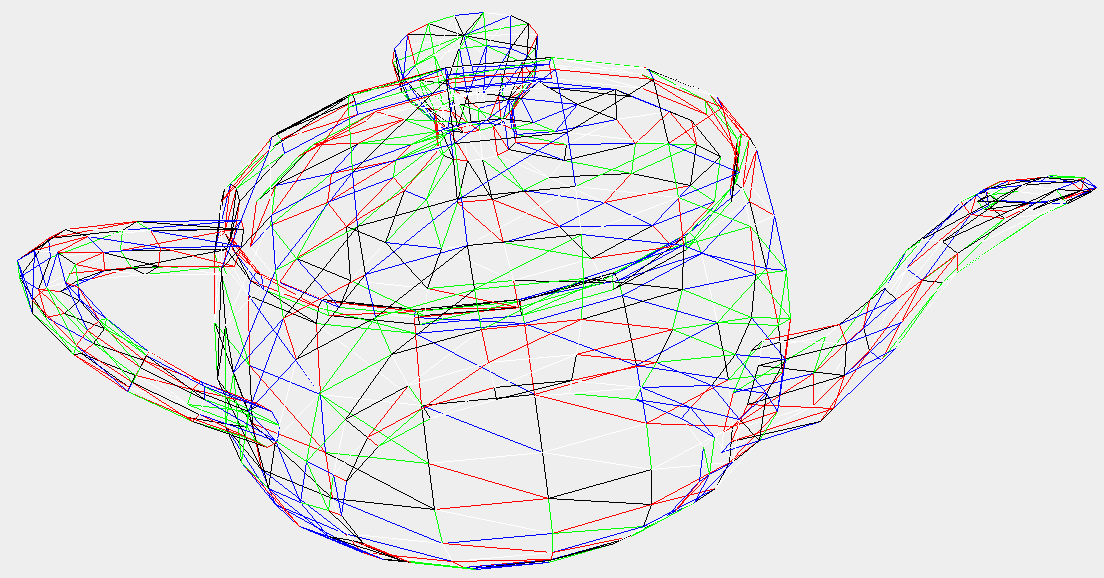
\includegraphics[scale=0.173]{teapot-reference.png}
\label{fig:teapot-reference}
}
\subfigure[Decomposition in Scala, rendered with Java graphics]{
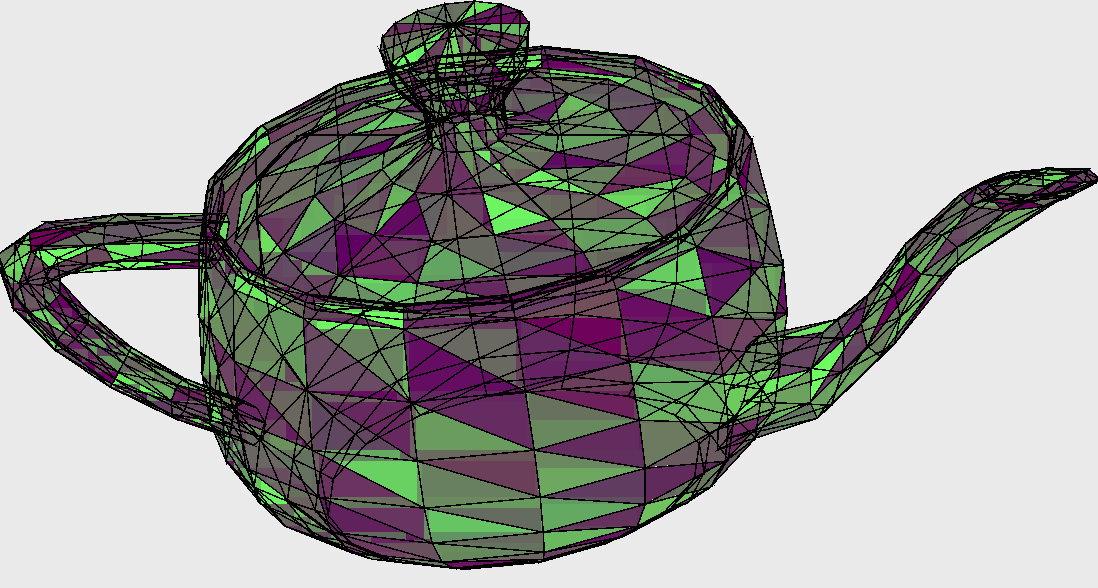
\includegraphics[scale=0.17]{teapot-java-canvas.png}
\label{fig:teapot-scala}
}
\subfigure[Decomposition in Scheme, rendered with appropriately positioned {\sc html} \textsf{div}
elements]{
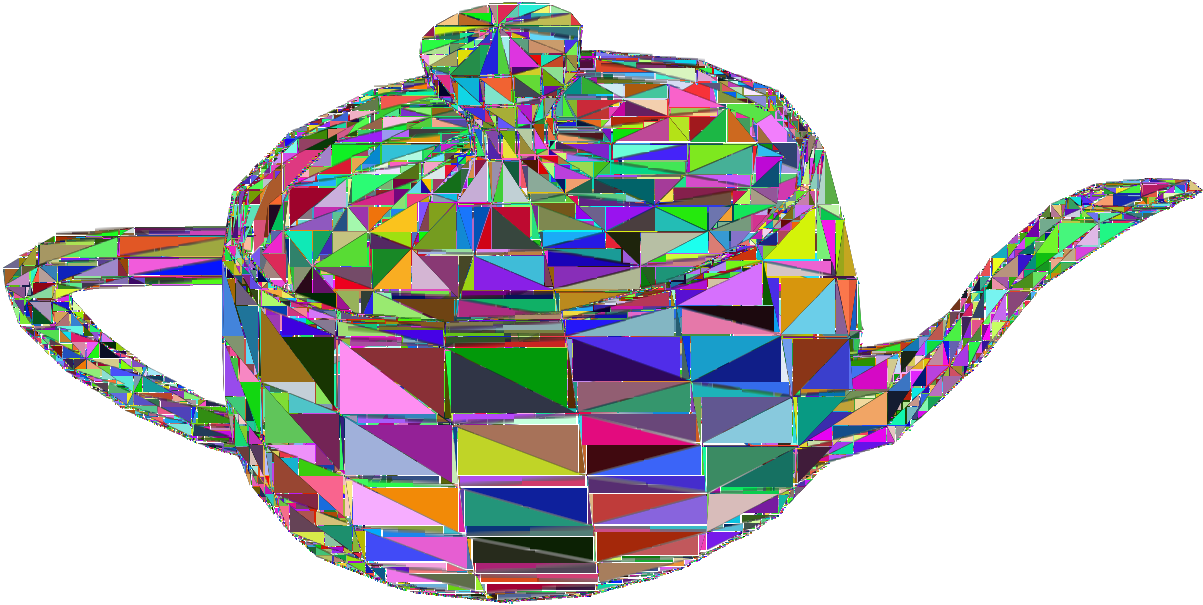
\includegraphics[scale=0.2]{teapot-html-divs.png}
\label{fig:teapot-html-divs}
}
\subfigure[Decomposition in Javascript, rendered with {\sc html5} graphics]{
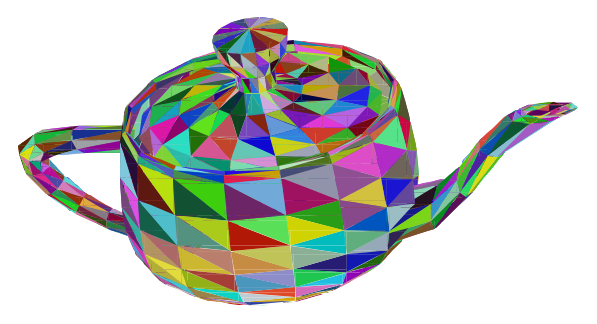
\includegraphics[scale=0.31]{teapot-html-canvas.png}
\label{fig:teapot-html-canvas}
}
\caption[]{Example results from the teapot exercise.}
\end{figure*}

The student's response was overwhelming. Even though it was made clear that
the exercise would not contribute to the final grade, the will to apply the
data processing techniques taught during the lectures motivated
the students to work very hard. The fact that they were instructed to use
their favourite language enabled them to focus on decomposing the problem 
in a series of testable calculation steps rather than meddling with the
intricacies of a pure functional language. Solutions where provided in
Scala, {\sc c\#}, Scheme, Javascript and Haskell. 
Example renderings produced by student programs can be seen in 
Figure~\ref{fig:teapots}.

\subsection{Teaching Map/Reduce}



\subsection{Student Projects}

\section{Conclusion}

Teaching the concepts of solving problems algorithmically can be a daunting
task~\cite{Futsc06}; especially more so, when the subjects are already in a
specific mindset. The assumption of the presented course was that imperative and
functional programming are really the two sides of the same coin; by focusing on
how students can apply rather than just be taught concepts of functional
programming using the, typically imperative, languages they already know, allows
them to better appreciate the strong points and weaknesses of each paradigm. In
our experience, the approach has been successful. Both throughout the initial
homework assignments and in their projects, the students demonstrated a high
degree of appreciation of functional programming concepts. Above all, we
believe that it was the hands-on approach through tough homework exercises
employed in this course that allowed students to sharpen their skills and
understand the concepts that were taught during the course.

\section*{Acknowledgements and Availability}

We would like to thank the course participants for their enthusiasm and
dedication. The source code to all student projects and the teapot
exercise can be found at (or linked from) \url{https://github.com/gousiosg/teapots}. 

\bibliography{paper}
\bibliographystyle{ieeetr}
\end{document}

